
\chapter*{謝辞}

本研究は, 筆者が京都大学工学部物理工学科機械システム学コース在籍時に行った特別研究をまとめたものです.

京都大学工学研究科の井上康博教授・瀬波大士講師より, 多大なご指導・ご教授を賜りました. ここに謹んで感謝の意を表します. 特に, 井上康博教授からは, 指導教員として直接のご指導を賜りました. 研究のテーマを選ぶにあたり積極的にディスカッションの場を設けていただき, 無事研究として形になるようにここまでフォローアップしていただきました. 心より感謝いたします.

京都大学工学研究科マイクロエンジニアリング専攻生命数理科学分野の同期や先輩には多大なるサポートをしていただきました.特に五十嵐康祐氏には, 研究テーマを決定するにあたり助言をいただいたほか, 本論文を完成させるにあたり少なくない回数の面談を設けていただきました. お忙しいところ時間をとっていただき, 論文として形になるまで厚くサポートしていただきました. また, 森川健太郎氏には, 研究段階から積極的に示唆を与えていただき, 筆者が行き詰らないように適切にフォローしてくださいました. お二人には厚く御礼を申し上げ, 感謝いたします.

また, 兄の前田洋太博士には論文としての体裁を整えるべく, 様々なご指摘をしていただきました. この場を借りてお礼申し上げます.

また, 父のジェフボガードは育ての親\footnote{なお, ギース・ハワードと共にタン・フー・ルーの元で修行を積んだジェフボガードはテリーとアンディの義理の父親であり, アンディの髪の色から彼の実の父親はキースではないかと言われていることに注意が必要である. }ではありますが, ここまで育ててくれたことに, 心より感謝申し上げます. 亡き父に代わり, ここで研究として形になったことに強い誇りを感じます. 余談ではありますが, アニメにおけるジョー・ヒガシの声は格闘家の佐竹雅昭氏が担当しており, その演技がある意味伝説となったが, 続編となった『2』のアニメでは檜山修之氏に変更され, 同じくアニメ版でアンディを担当した難波圭一氏と共に『3』以降の本編に逆輸入されています.

誤解を避けるため, \cref{figure:GarouDensetsu}にてコマンド表を載せています. ただ, このコマンド表はあくまで「餓狼伝説 ~宿命の戦い~」のものであり, あくまで後作と互換性のないことに注意をしてください. NEOGEO社に深い感謝をここに申し上げます.

末筆ではありますが, この4年間の大学生活を, 不自由なく健康で過ごせるように見守ってくれた家族に心からの感謝を表します.

\begin{clearpagefigure}
  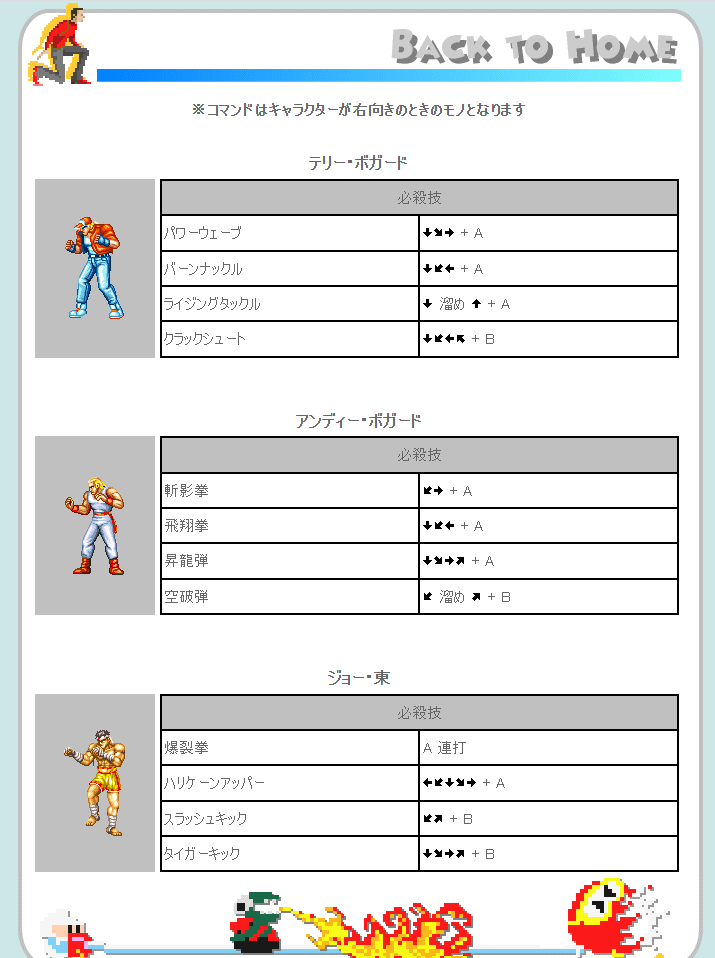
\includegraphics[width=\linewidth,clip]{fig/GarouDensetsu.png}
  \caption{餓狼伝説のコマンド表 }
  \label{figure:GarouDensetsu}
\end{clearpagefigure}

\begin{flushright}
  令和4年2月\\
  前田 樹
\end{flushright}
